\section{Introduction}\label{sec:introduction}
In the era of Information Technology, the usage of softwares and applications are growing day by day and have become an important part of our lives. This makes the software industry one of the largest industries on the world and many others companies are built around the development of softwares. With the growing usage of softwares, software development process has changed drastically and currently more solution oriented. Nowadays, the entire focus is making the software development process fast, less complex and more human-friendly. 
\newline\newline One of the approach to reduce the complexity of software development is abstraction and separation of concerns \cite{modeltransform}. In recent times, software modeling has become an effective way for implementing this principle. In traditional approach, developers manually writes programs and checks the specifications realted to software models, which is often costly, incomplete, informal and carries a major risk of failure. On the contrary, model-driven software development (MDSD) approach improves the way softwares are built by moving the focus from programming language code and representing the essential aspects of software in the form of software models. It increases the reduces the development costs and increases the reusability and maintainability of software. The objective of MDSD \cite{modeltransform} is to increase productivity and reduce time-to-market by enabling development at a higher level of abstraction and by using concepts closer to the problem domain at hand, rather than the ones offered by programming languages. 
\newline\newline The core idea of MDSD approach is based on models, modeling and model transformations. In this approach, developers depits the real world system under discussion in the form of models with certain level of abstraction. These models are used to form the problem domain and the relationships between them helps to form the solution domain. Models can be changed to represent different state/view of the system. But, it is necessary to change between different states of a system with equivalent level of abstarction by ensuring their overall consistency. This phenomenon is handled by model transformation. This certainly increases the developers productivity and the quality of the models.

\textit{Bidirectional transformation} (denoted by "bx") is a technique used to synchronize two (or more) instance of different meta-models. Both models are related, but don't necessarily contain the same information. Changes in one model thus lead to changes in the other model \cite{bx-grace}. Bx makes sure that two models that can change over time have to be kept constantly consistent with each other.
\newline\newline\textit{Bidirectional transformation} is used to deal with scenarios like:
\begin{itemize}
	\item {change propagation to the user interface as a result of underlying data changes}	
	\item {synchronization of business/software models}
	\item {refreshable data-cache incase of database changes}
	\item {consistency management between two artifacts by avoiding data loss}
\end{itemize}
    and many more....
\newline\newline Bx community has been doing research and development work in many fields like software development, database, mathematics and much more to increase awareness and to reach more people \cite{bx-dagstuhl}\cite{bx-grace}. As a result, many kinds of bx tools are being developed, e.g., eMoflon \cite{emoflon-part4}, Echo \cite{echo}. These bx tools are based on various approaches, such as graph transformations, bidirectionalization, update propagations \cite{bx-community} and can be used in different areas of application.

\subsection{Problem Statement}\label{subsec:probstmt}
\textit{Bidirectional transformation} is an emerging concept. In the past, many efforts have been made by conducting international workshops, seminars and through experiments conducted by developers / bx community to identify its potential. Also, in addition to the development of bx tools and bx language, benchmarks are being created for bx tools for systematic comparison \cite{benchmark-BX}.
\newline\newline  Although a significant amount of work has been done in this field, some basic problems still remain:
\begin{itemize}
	\item {\textbf{Reachability: } Reachability to relevant communities is not significant due to the absence of a common vocabulary for bx across research disciplines \cite{bx-theoryandappl}. Seminars are still conducted for exchanging ideas in different communities to define a common vocabulary of terms and properties for bx \cite{bx-dagstuhl}.}	
	\item {\textbf{Applicability: } Bx tools and their applicability is still not widely known even in the developers' communities. Many developers and researchers are still using non-bx transformation tools to achieve properties which can be easily supported by bx-tools \cite{bx-theoryandappl}. This is because of the existing conceptual and practical challenges associated with configuring/trying a bx-tool for knowing its potential, building software systems using bx-tools, etc.}
	\item {\textbf{Demonstrator: } Absence of a simple yet interactive bx tool demonstrator to depict the potential of \textit{bidirectional transformation} over preferred non-bx tool demonstrators among developers' and researchers' communities \cite{bx-theoryandappl}.}
\end{itemize}

\subsection{Solution Idea}\label{subsec:solution}
To solve the problems as described in Section \ref{subsec:probstmt}, in this thesis, my goals are as follows:
\begin{itemize} 
\item {Design and implement an interactive demonstrator.} 
\item {Spreading the basic concepts of bx to a wide audience and making them accessible and understandable.}
\end{itemize}
An existing bx tool will be used as a part of the demonstrator to realize \textit{bidirectional transformation}. The final prototype will be interactive and easily accessible to users to help them understand the potential, power and limitations of bx.

\subsection{Approach Overview}\label{subsec:approach}
My approach for providing a solution to the problems described in Section \ref{subsec:probstmt}  consists of various stages which focuses on designing and implementing a successful bx tool demonstrator for mitigating the problems as shown in figure~\ref{fig:Approach_Overview}. 

\begin{figure}
	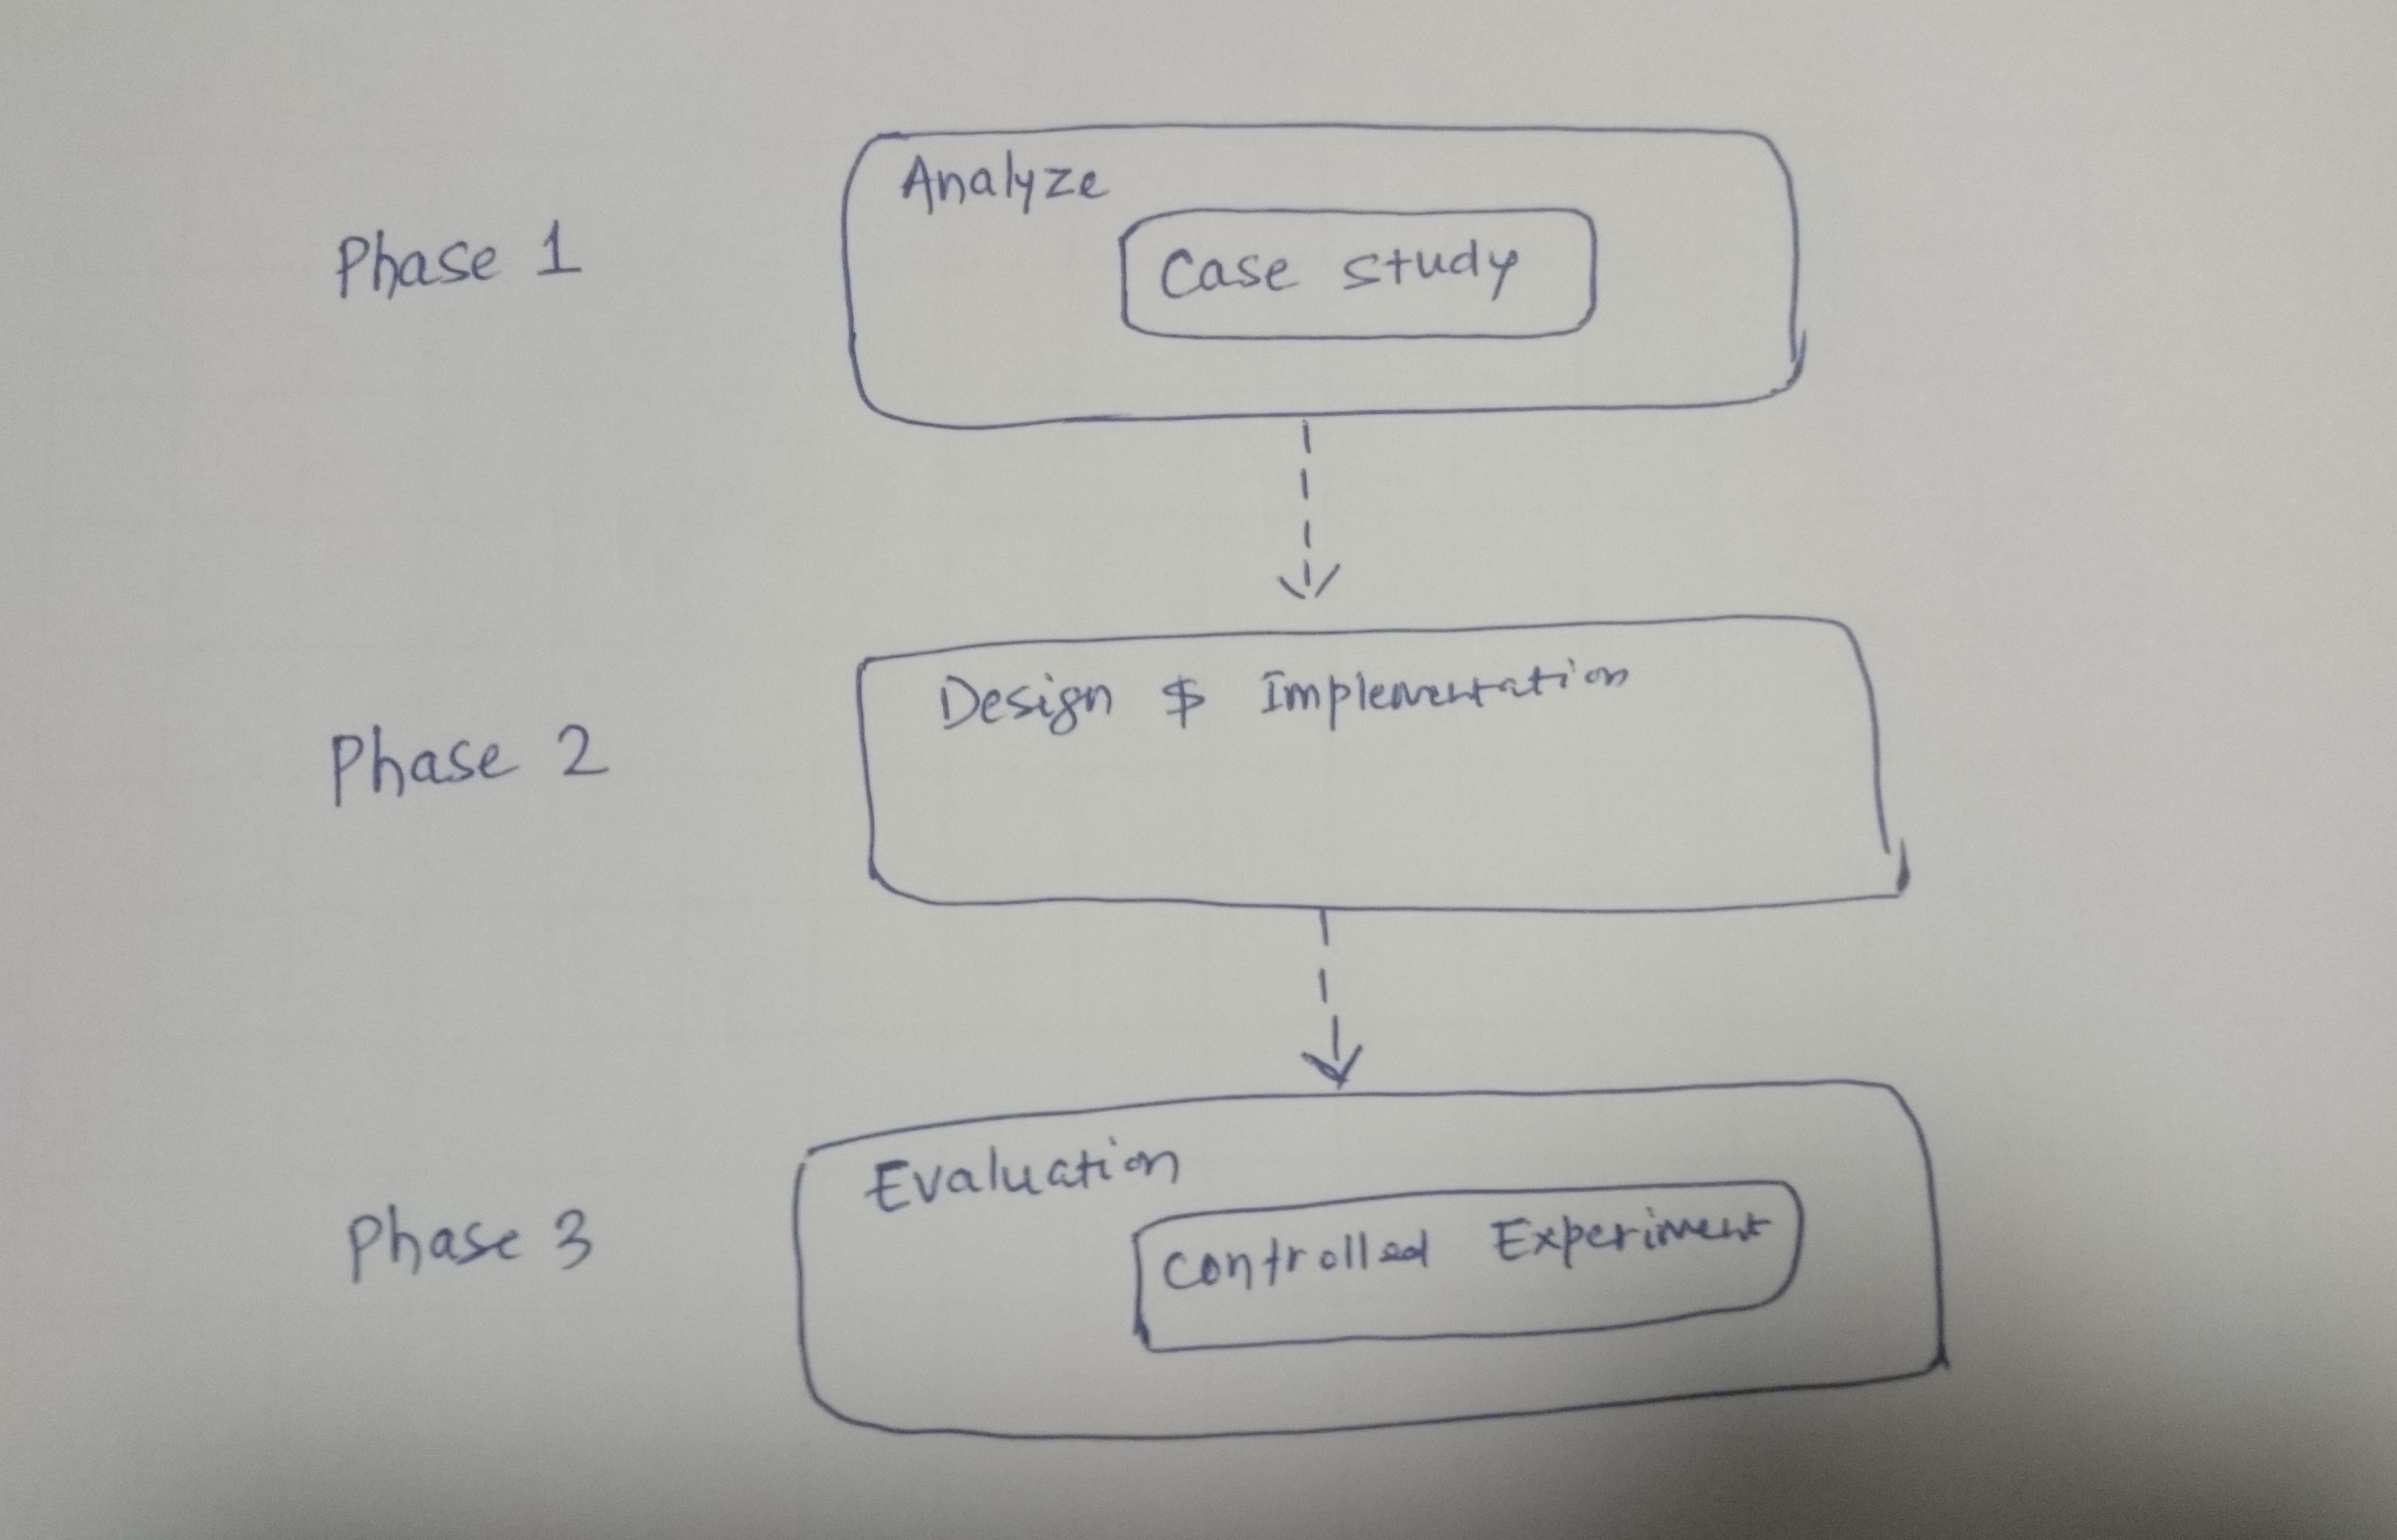
\includegraphics[width=1\textwidth]{figures/Approach_Overview}
	\caption{Approach Overview}
	\label{fig:Approach_Overview}
\end{figure}

\paragraph{Analysis}
This stage is based on the research method called Case Study \cite{semethods}. In any research, there could be many cases and each case could focus on a number of different research questions, each of which leads to a different direction in developing solution strategies \cite{semethods}. Hence, this method aims at selecting cases that are most relevant to the research and research questions are pinned down to the exact problems in hand. 
\newline\newline Initially, the case study was based on the existing work/research done on bx, existing tools available in the market, flexibility in usage, time and technical expertise required to use these bx tools, and the implementation of these tools in different areas. With the initial study and knowledge gathered, I have divided the problems into following relevant cases and associated research questions:\\\\
\textbf{Case: Demonstrator}
\begin{itemize}
\item {\textbf{\textit{RQ1}} -- What are the core requirements for implementing a successful bx demonstrator ?}
\item {\textbf{\textit{RQ2}} -- What kind of interactivity and to what extent is it required in the bx demonstrator ?}
\item {\textbf{\textit{RQ3}} -- Which goals can be particularly well addressed in a bx demonstrator and why ?}
\end{itemize}
\textbf{Case: Applicability}
\begin{itemize}
\item {\textbf{\textit{RQ4}} -- To what extent is such a bx demonstrator reusable?}
\\RQ4 can be split into the following sub-questions:
\\\textbf{\textit{RQ4.1}} -- Is the implementation of the demonstrator bx tool-specific ?
\\\textbf{\textit{RQ4.2}} -- Is the implementation of the demonstrator example-specific?
\\\textbf{\textit{RQ4.3}} -- What part(s) of the demonstrator can be reused in implementing a different example ?
\end{itemize}
\textbf{Case: Reachability}
\begin{itemize}
\item {\textbf{\textit{RQ5}} -- Is it possible to teach the concepts of bx through a demonstrator ?}
\item {\textbf{\textit{RQ6}} -- Does an interactive GUI helps an user to increase his/her understanding of bx concepts ?}
\end{itemize}
All of my work is directly or indirectly related to the above research questions.

\paragraph{Design and Implementation}
This stage is consist of all the steps related to designing and implementing the demonstrator by keeping a focus on the research questions.
\newline\newline First step was to choose a bx-tool for my demonstrator. Based on the gathered information and taking account implementation related issues, I have chosen a bx-tool to be used as a part of the demonstrator to realize bx. Section \ref{subsec:bxtoolselection} explains the process in detail.
\newline\newline Secondly, I have constructed a few examples which can be implemented covering the requirements and showing the usability of bx tools through demonstrator. Then, taking account the availabilities of resources and usability factor, I finally chose the best suitable example to implement and build the final prototype. Section \ref{subsec:examples} describes list of all the examples.
\newline\newline Next step was to set up the entire application framework for implementing the demonstrator. First, I did some research by going through materials on software design patterns and web application architecture. Then, I prepared a few proof of concepts(POC) for checking the feasibilty of the architecture designs before finalising my application framework. Section \ref{subsec:architecturedesign} explains the process in detail.

\paragraph{Evaluation} 
This stage is based on the research method called Controlled Experiments \cite{semethods}. This experiment is based on one or more hypothesis, which guide all steps of the experimental design, deciding which variables to include and how to measure them. So, it is an investigation of one or more hypothesis where one or more independent variables are manipulated to measure their effect on one or more
dependent variables. Finally, data is collected and analyzed to measure the outcome. Section \ref{subsec:evaluation} explains the process in detail.

\subsection{Structure}\label{subsec:structure}
This document is structured as follows: 

Chapter 1 (introduction) contains the introduction and motivation about the thesis with a solution strategy.

Chapter 2 discusses the related terminologies with respect to bidirectional transformation.

Chapter 3 describes the requirements for implementing a successful bx demonstrator.

Chapter 4 explains the related work that has been done on bx in last few years and the related problems.

Chapter 5 describes all the high-level concepts of my implementation work in brief with related diagrams.

Chapter 6 provides the in-depth details of each implementation layer along with UML diagrams.

Chapter 7 presents a walkthrough of the application from UI perspective.

Chapter 8 contains the feedback from user groups, evaluation results and learning goals(based on research questions).

Last chapter summarizes all the work which was done as part of this thesis and draws useful conclusions followed by future work.

\section{Foundation}\label{sec:foundation}
This chapter describes some commonly used terminologies with respect to bx and their definitions in the software industry. These definitions will help the reader in understanding the further chapters.

As already mentioned, \textbf{"bx is a technique to maintain consistency(synchronization) between two(or more) related models"}.

\paragraph{Model}is an artefact or external representation of reality which reflects certain relevant aspects of a real system. It is denoted as "M".
\begin{itemize}
\item {Artefact, because it is something artificial, not real.}
\item {External representation, because it can be a drawing, a physical object or software generated on a computer.}
\item {Certain relevant aspects, because it contains some properties related to the real system.}
\end{itemize}
A model depicts the structure and/or behavior of the system under discussion from a certain viewpoint and at a certain level of abstraction which helps in managing and understanding the complexities of a system \cite{uml} \cite{mdsd}.
\newline\newline\textit{Example:} In my demonstrator, the example that I have implemented has two models, e.g. Kitchen and Grid which represents the reality "Kitchen". A relation between reality and model is shown in Table~\ref{tab:Model and Reality}.
\begin{table}
	\centering	
	\begin{tabular}{|p{3cm}|p{3cm}|p{9cm}|}
		\hline
		\rowcolor[gray]{.8}	
		\textbf{Reality} & \textbf{Model} & \textbf{Aspects Covered} \\
		\hline
		Kitchen & Kitchen Model & 
		\begin{itemize}
			\item Area of a kitchen as a white space
			\item 4 Walls of a kitchen
			\item contains the objeccts of a kichen
			\item Creating, Moving, Deletion of kitchen objects
		\end{itemize}\\
		\hline
		Kitchen & Grid Model & 
		\begin{itemize}
				\item Area of a kitchen as a block structure
				\item 4 Walls of a kitchen
				\item contains the objeccts of a kichen
				\item Creating, Deletion of kitchen objects
		\end{itemize}\\
		\hline					
		
	\end{tabular}
	\label{tab:Model and Reality}
	\caption{Model and Reality}
\end{table}

\paragraph{Modeling} is the process which allows a developer to specify, visualize and capture a variety of important characteristics of a system in corresponding models which helps in decision making in all the development stages \cite{uml}. Nowadays, Unified Modeling Language (UML) \cite{uml} is used to visualize models in an object-oriented fashion.
\newline\newline\textit{Example:} In my demonstrator example, the process of identifying and constructing the "Grid Model" with the characteristics that is required for the task. A basic model of the "Grid Model" is shown in figure~\ref{fig:Modeling_Example}.

\begin{figure}
	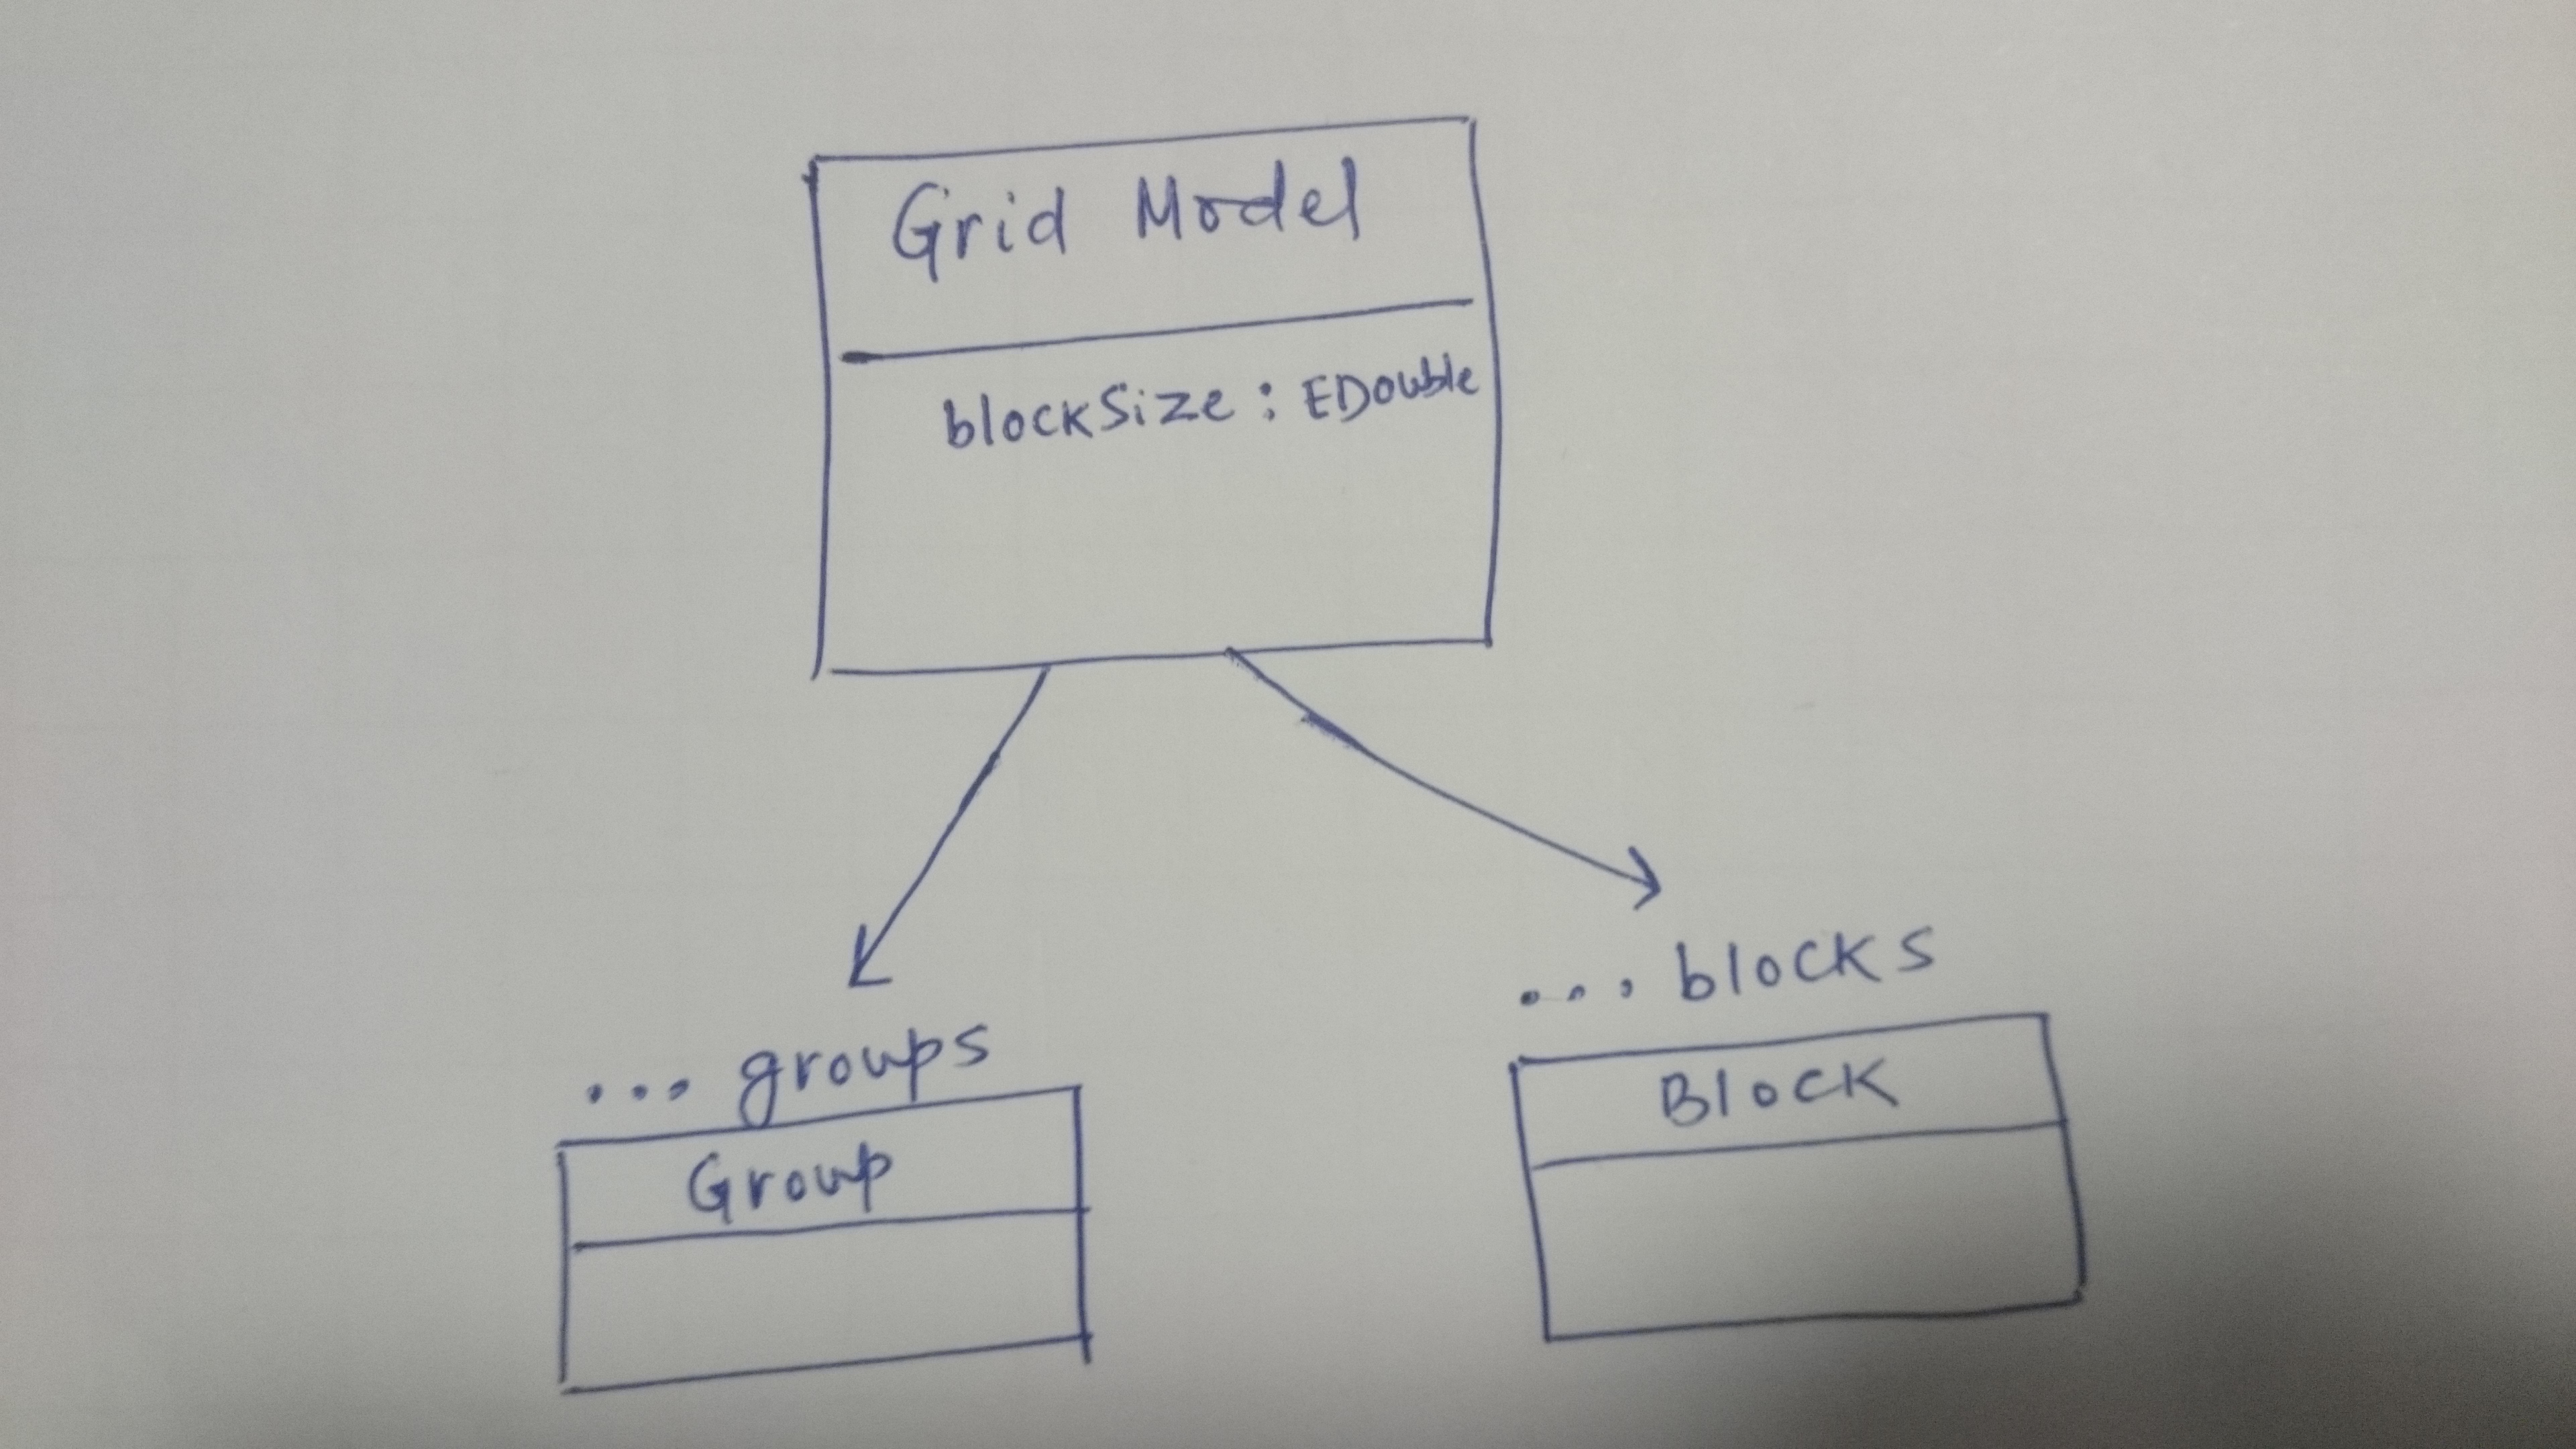
\includegraphics[width=1\textwidth]{figures/Modeling_Example}
	\caption{Modeling Example}
	\label{fig:Modeling_Example}
\end{figure}

\paragraph{State} denotes the condition of an artefact at any given point of time.

\paragraph{Delta} is the change done to one or more properties of an artefact which causes the transformation. It is denoted as $\delta$.
\newline\newline\textit{Example:} In my demonstrator example, deltas related to the "Kitchen Model" are described in Table~\ref{tab:Examples of Delta}. 
\begin{table}
	\centering	
	\begin{tabular}{|p{5cm}|p{10cm}|}
		\hline
		\rowcolor[gray]{.8}	
		\textbf{Model} & \textbf{Delta ($\delta$)} \\
		\hline
		Kitchen Model & 
		\begin{itemize}
			\item Creating a new Item
			\item Deleting an existing Item
			\item Moving an Item
		\end{itemize}\\
		\hline				
		
	\end{tabular}
	\label{tab:Examples of Delta}
	\caption{Examples of Delta}
\end{table}

\paragraph{Transformation} is the process in which an artefact undergo a change from one state to another. 
\newline\newline\textit{Example:} In my demonstrator example, creating a delta($\delta$) in the "Kitchen Model" will cause a transformation. Refer Figure~\ref{fig:Transformation_Diagram}.

\begin{figure}
	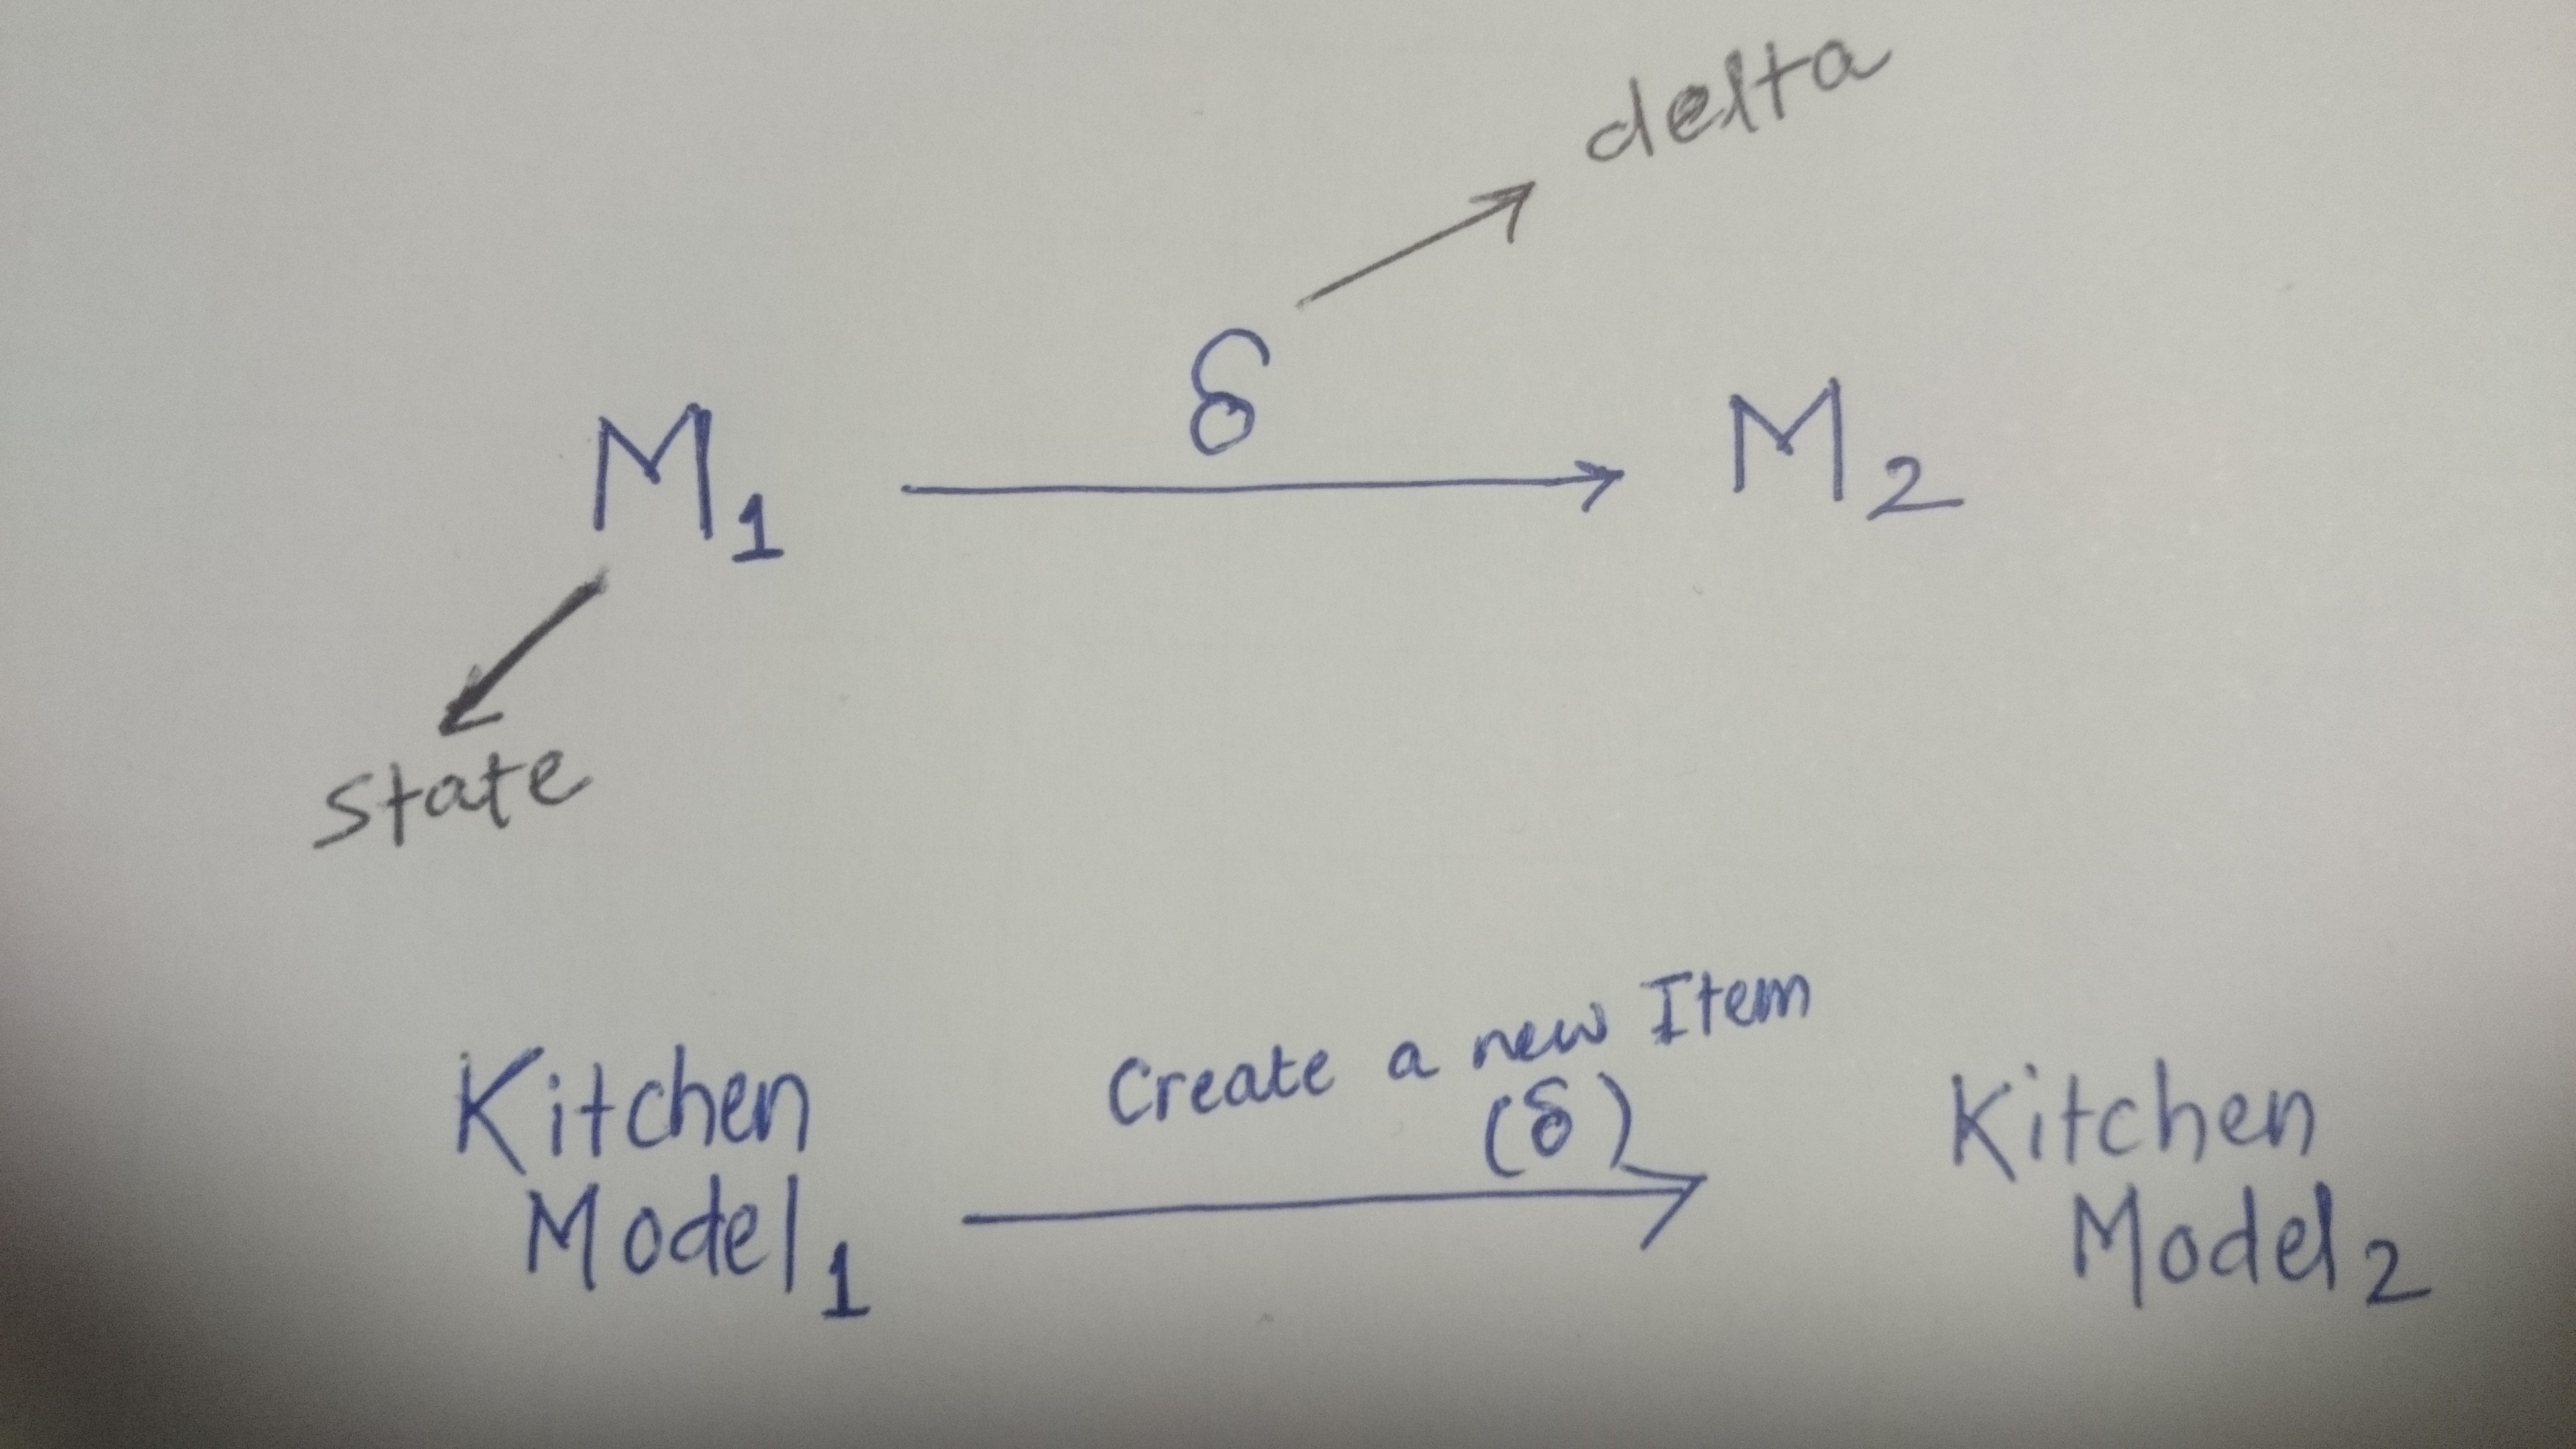
\includegraphics[width=1\textwidth]{figures/Transformation}
	\caption{Transformation}
	\label{fig:Transformation_Diagram}
\end{figure}

\paragraph{State Space} describes all the states of an artefact and all the deltas which lead from one state to another. Refer Figure~\ref{fig:StateSpace_Diagram}.
\begin{figure}
	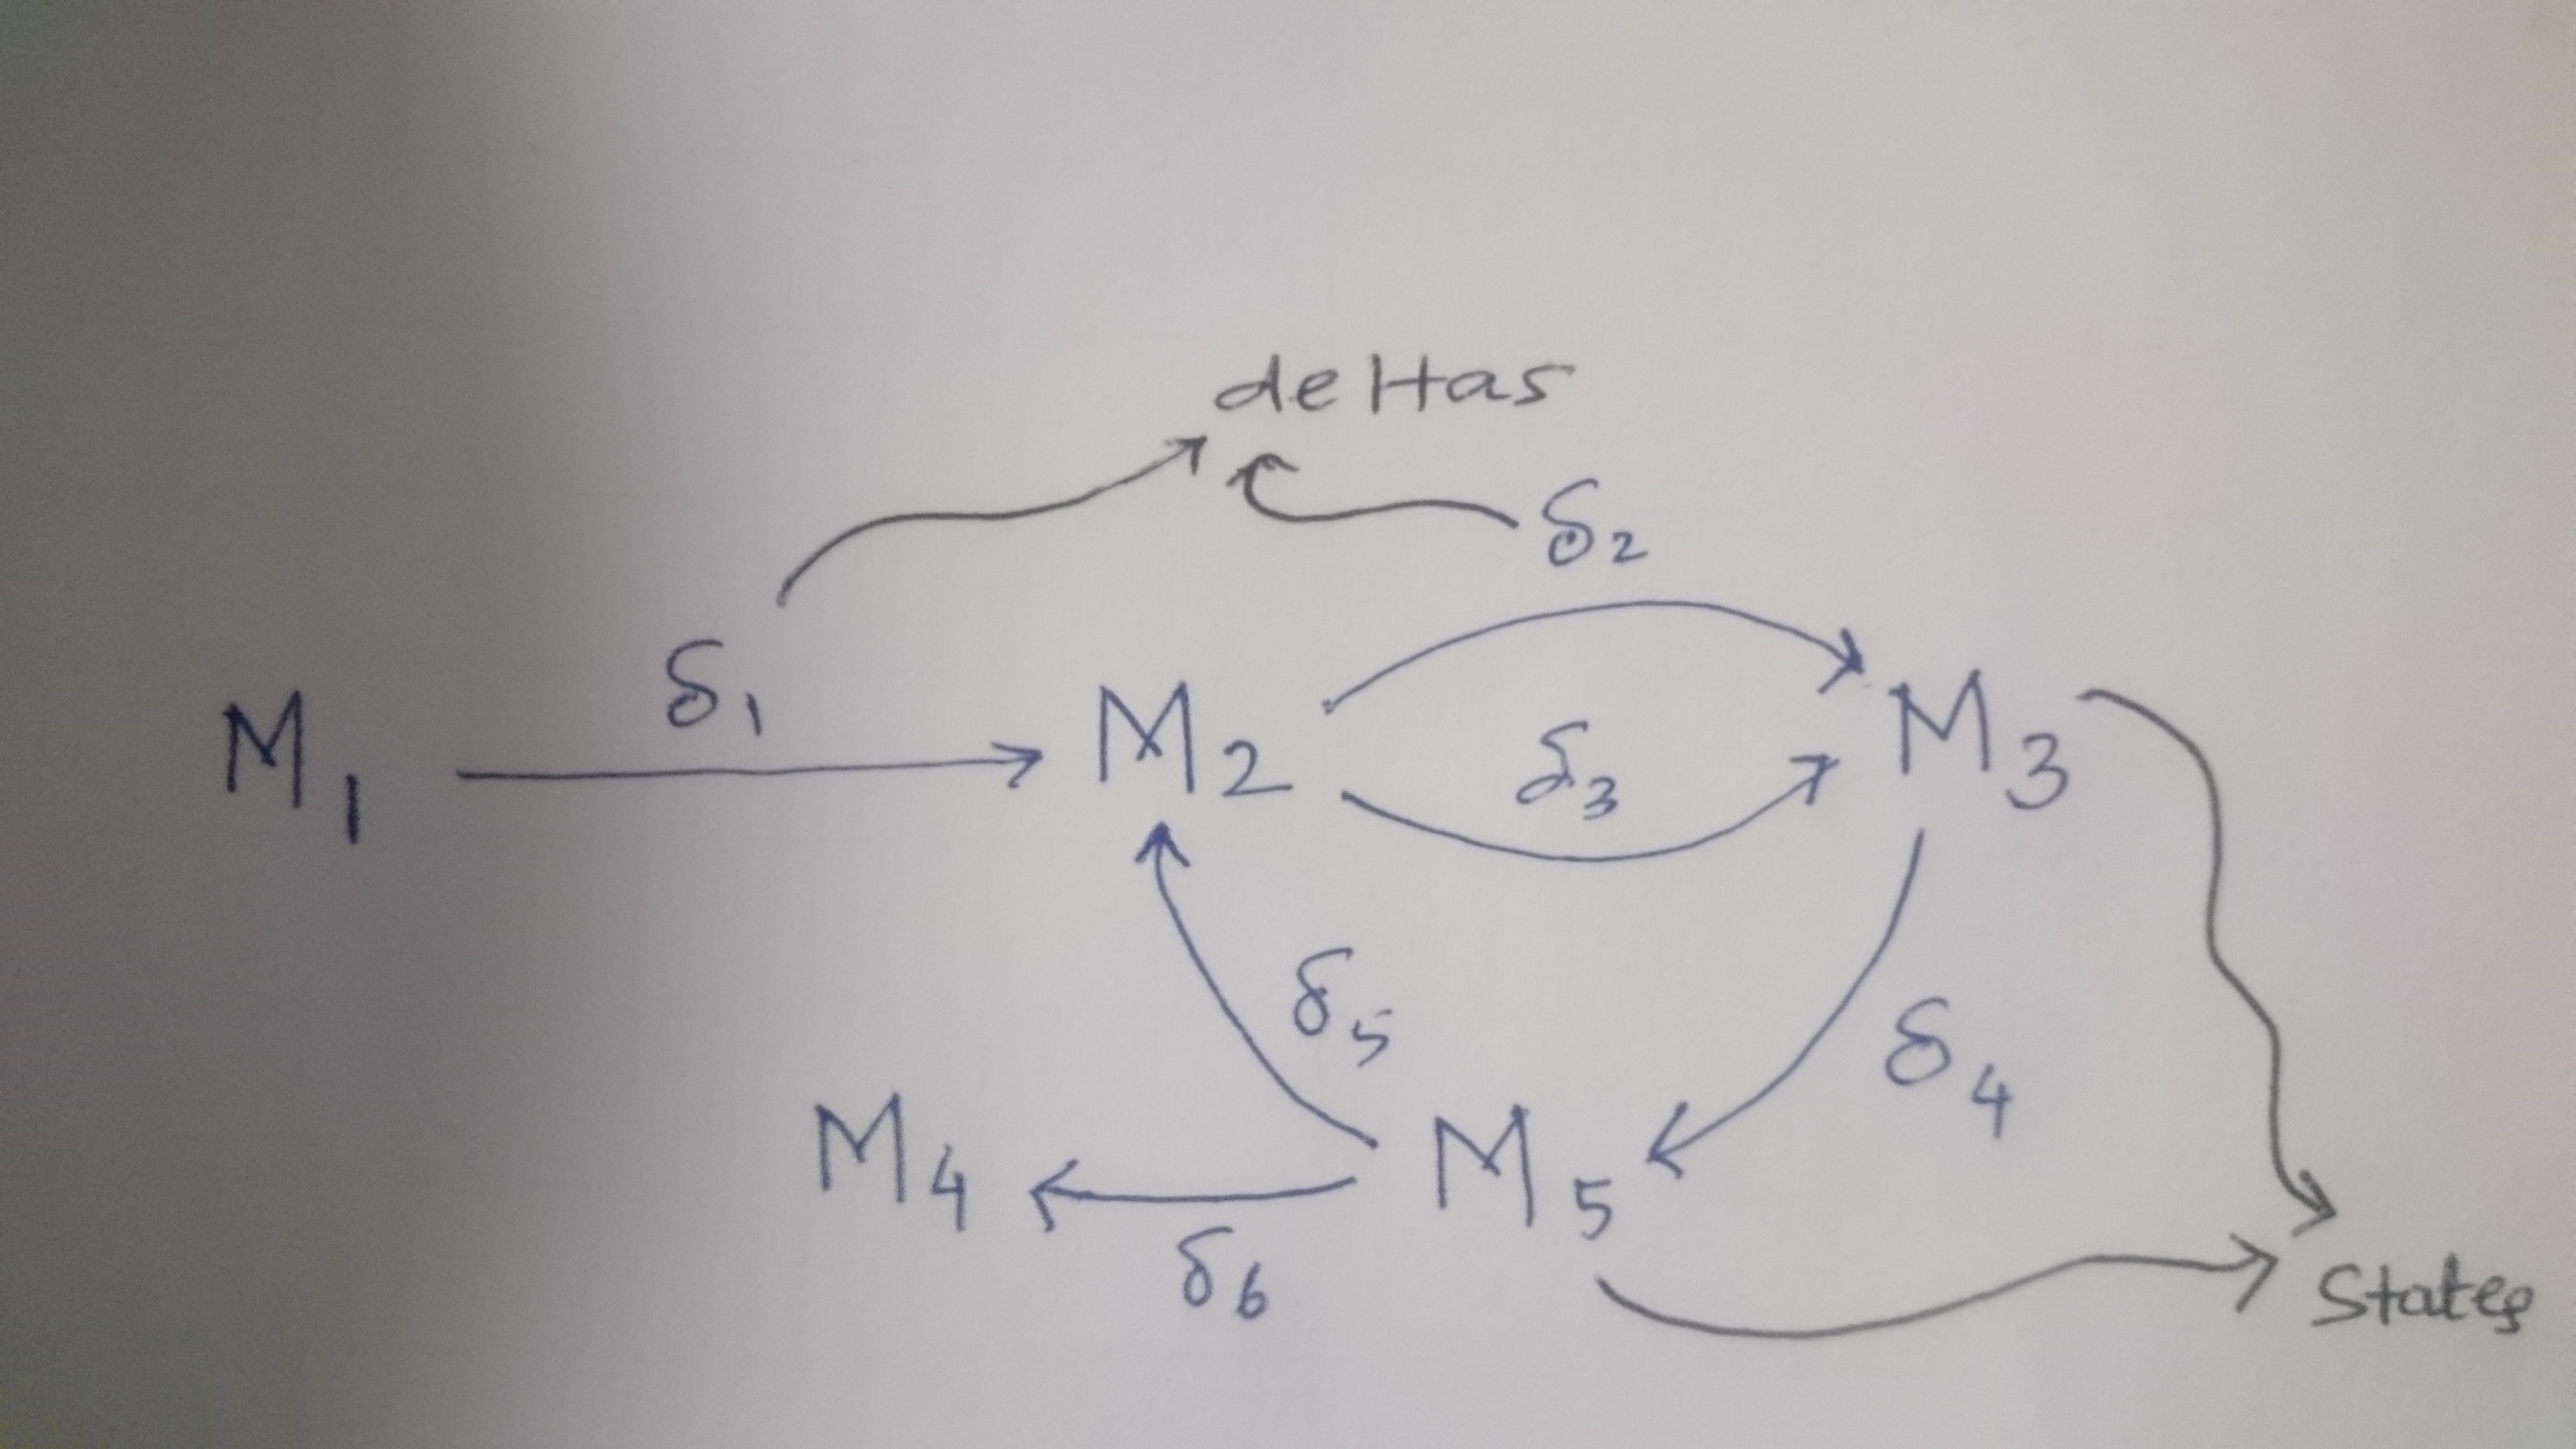
\includegraphics[width=1\textwidth]{figures/State_Space}
	\caption{State Space}
	\label{fig:StateSpace_Diagram}
\end{figure}

\paragraph{Consistency} In layman's term, consistent is a state which always involves 2 or more objects/artefacts but doesn't involve ambiguity between them. This is the most important part of the model transformation and the entire focus revolves around it. To be consistent with each other the models have to be inline with respect to their states. Changes in one model may or may not cause any change in other model but their states must not contain any contradiction. 

\paragraph{Unidirectional vs.Bidirectional Transformation}  Unidirectional is the simplest one out of all kinds of transformation. It always takes one type of input and produces same type of output \cite{wiki-transformation}. The concept of consistency is very simple as the input model is consistent with the output model, only.
\newline Whereas, bidirectional transformationis a pair of transformation which takes place in both forward and backward direction. One model can be input sometimes and output at some other time. The concept of consistency is relatively complex as more than one model and the models must be kept consistent. Source model ($M_{S}$) is transformed to target model ($M_{T}$) in forward transformation and vice-versa in backward transformation. It is denoted by "BX". 
\newline Figure~\ref{fig:BX_Diagram} describes the concept in detail.
\begin{figure}
	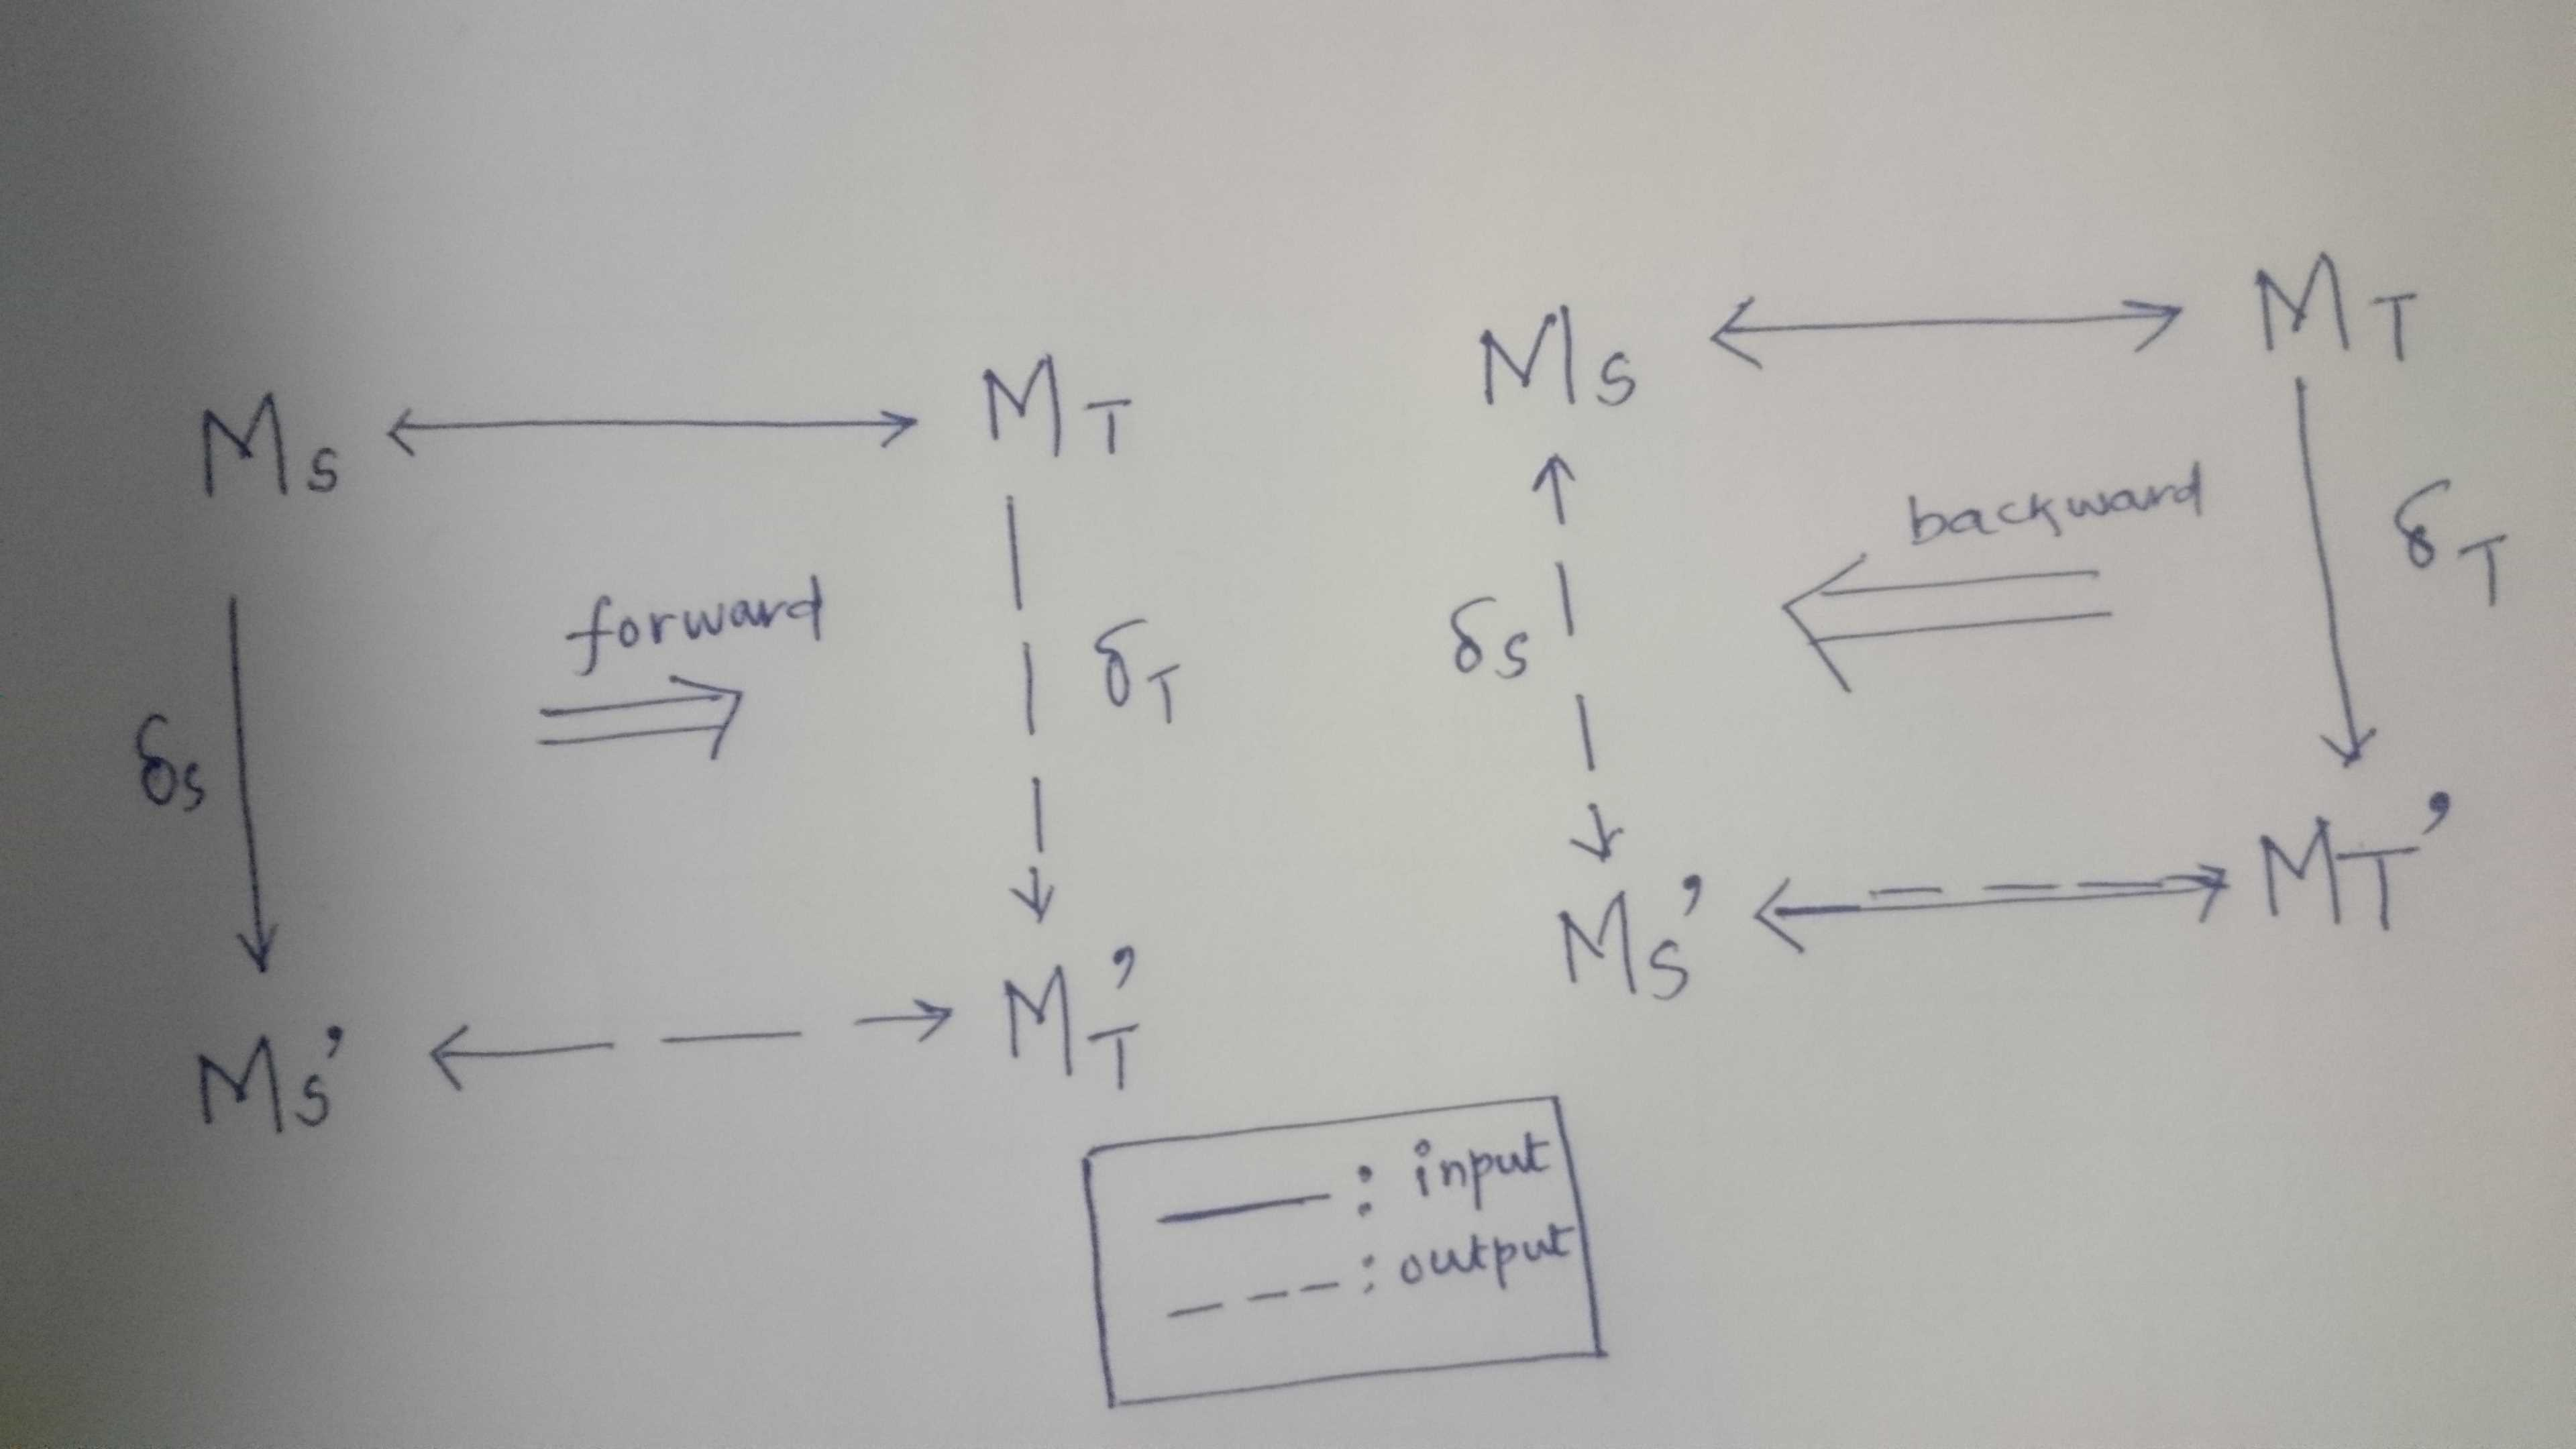
\includegraphics[width=1\textwidth]{figures/BX}
	\caption{Bidirectional Transformation}
	\label{fig:BX_Diagram}
\end{figure}

\paragraph{Bijective vs.Bidirectional Transformation}  


 



